%% LaTeX2e class for student theses
%% sections/apendix.tex
%% 
%% Karlsruhe Institute of Technology
%% Institute for Program Structures and Data Organization
%% Chair for Software Design and Quality (SDQ)
%%
%% Dr.-Ing. Erik Burger
%% burger@kit.edu
%%
%% Version 1.1, 2014-11-21


\iflanguage{english}
{\chapter{Appendix}}    % english style
{\chapter{Anhang}}      % german style
\label{chap:appendix}

\section{ }
\label{sec:app:}

\textbf{2 Cylinder const speed BC}
\begin{figure}[H]
		%\centering
            \begin{subfigure}{0.49\textwidth}
                  \flushleft
                  \scalebox{0.42}{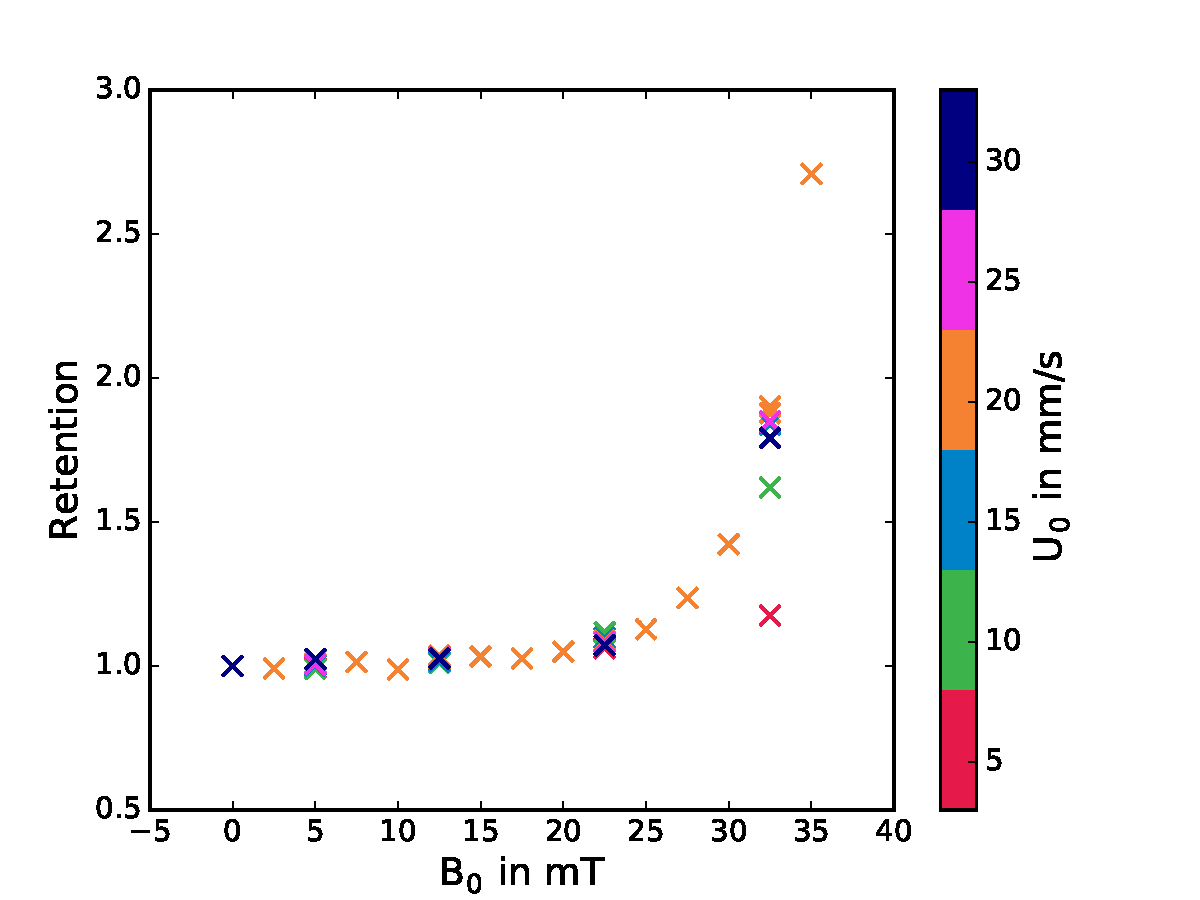
\includegraphics{figures/B0_Rp_30_U0_var_2Cylinder_constBC.pdf}}
                  \caption{Results for $R_{p}$=30\,nm and $U_{0}$ variable}\label{subfig:tw_constBC_U0_var}
          \end{subfigure}\hfill
        \begin{subfigure}{0.49\textwidth}
                \flushright
                \scalebox{0.42}{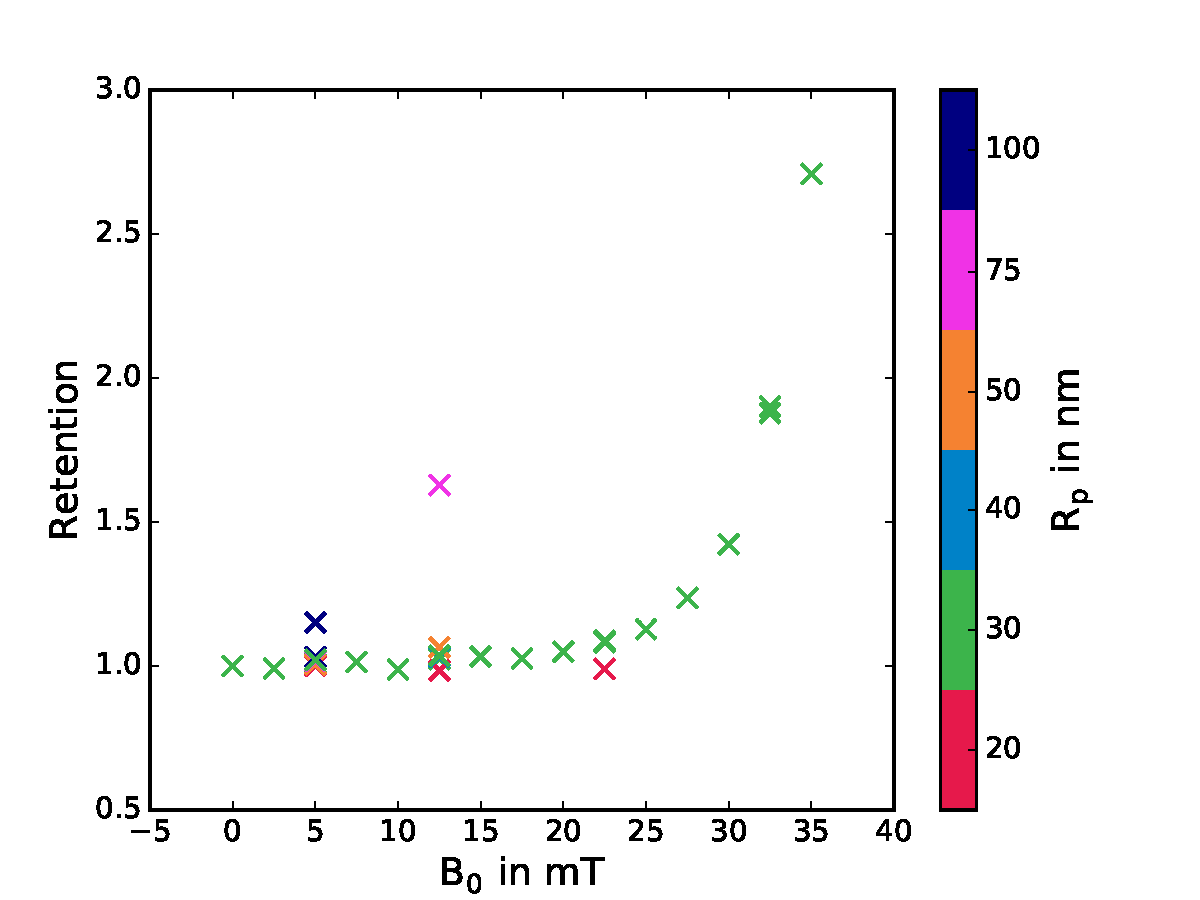
\includegraphics{figures/B0_Rp_var_U0_20_2Cylinder_constBC.pdf}}
                \caption{Results for $R_{p}$ variable and $U_{0}$=200\,\textmu m/s}\label{subfig:tw_constBC_Rp_var}
        \end{subfigure}
        \\       
          \caption[Parameter study results of the simulated retention of nanoparticles on two wires with a constant velocity boundary condition at the channel walls]{Parameter study results of the simulated retention of nanoparticles on two wires with a constant velocity boundary condition at the channel walls: the retention is plotted against the magnetic flux density $B_{0}$ in mT of the external applied magnetic field, the colorbar indicates the values of the varied parameter while the other parameters where held constant}
        \label{fig:tw_param_res_constBC}
  \end{figure}
        
\textbf{4 Cylinder const speed BC}
\begin{figure}[H]
		%\centering
            \begin{subfigure}{0.49\textwidth}
                  \flushleft
                  \scalebox{0.42}{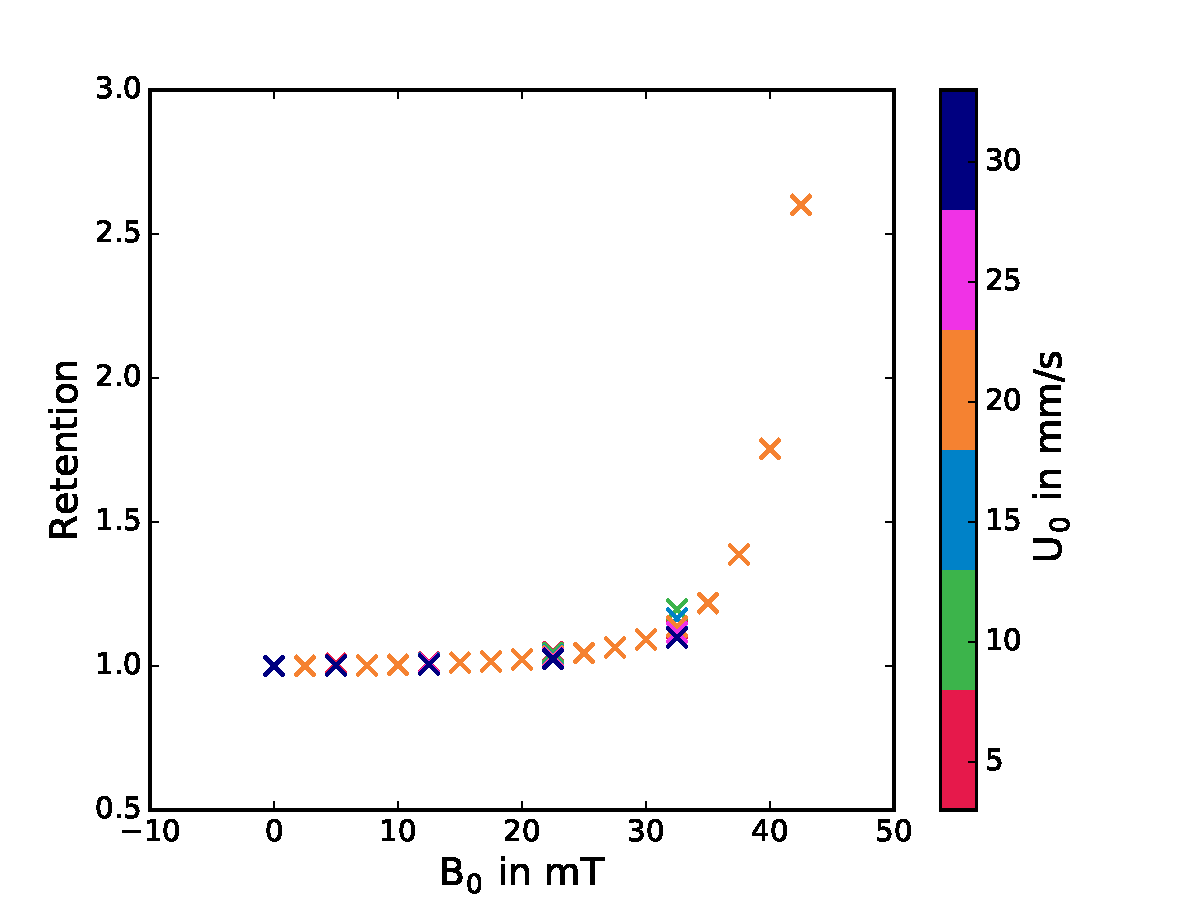
\includegraphics{figures/B0_Rp_30_U0_var_4Cylinder_constBC.pdf}}
                 \caption{Results for $R_{p}$=30\,nm and $U_{0}$ variable}\label{subfig:fw_constBC_U0_var}
          \end{subfigure}\hfill
        \begin{subfigure}{0.49\textwidth}
                \flushright
                \scalebox{0.42}{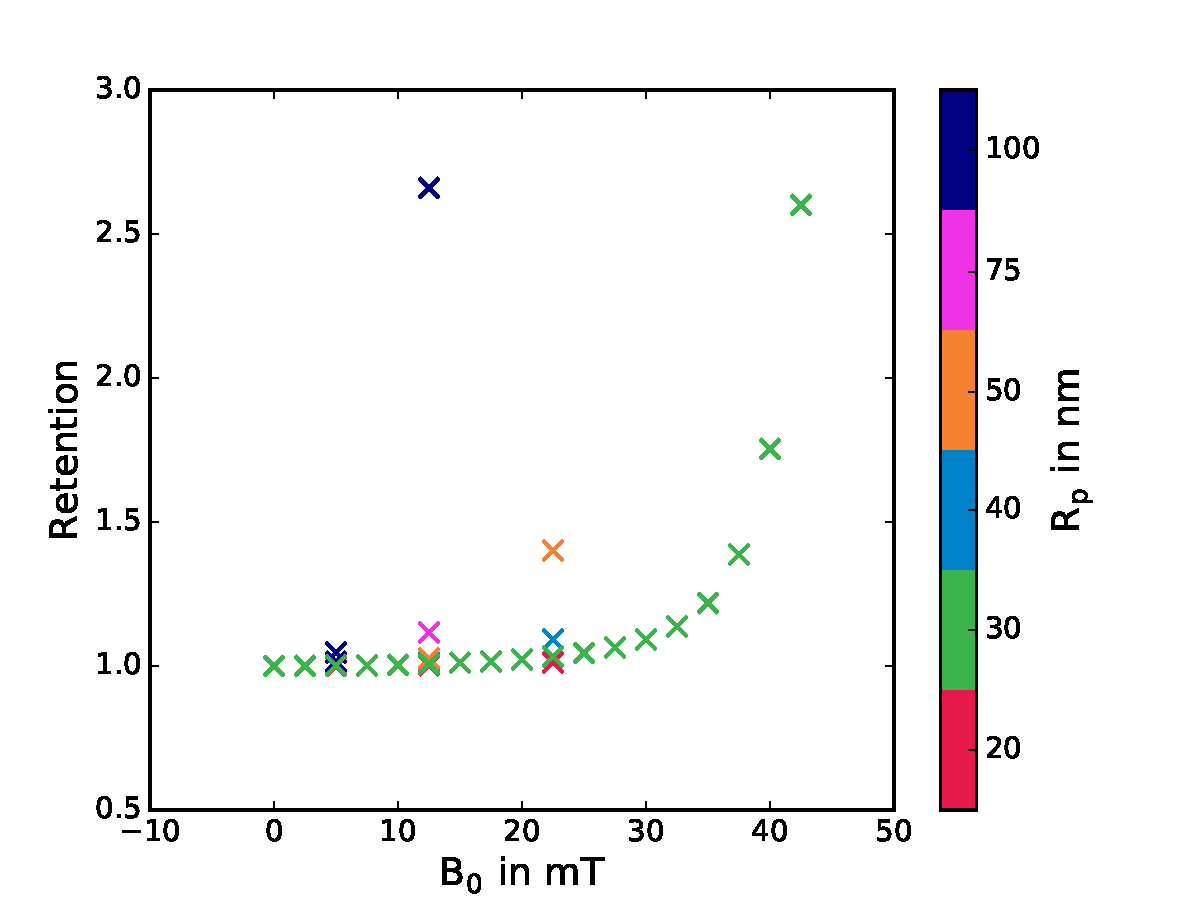
\includegraphics{figures/B0_Rp_var_U0_20_4Cylinder_constBC.pdf}}
                 \caption{Results for $R_{p}$ variable and $U_{0}$=200\,\textmu m/s}\label{subfig:fw_constBC_Rp_var}
        \end{subfigure}
        \\
        
          \caption[Parameter study results of the simulated retention of nanoparticles on four wires with a constant velocity boundary condition at the channel walls]{Parameter study results of the simulated retention of nanoparticles on four wires with a constant velocity boundary condition at the channel walls: the retention is plotted against the magnetic flux density $B_{0}$ in mT of the external applied magnetic field, the colorbar indicates the values of the varied parameter while the other parameters where held constant}
        \label{fig:fw_param_res_constBC}
  \end{figure}
        

        
\begin{figure}
		\centering
            \begin{subfigure}{0.49\textwidth}
                  \flushleft
                  \scalebox{0.42}{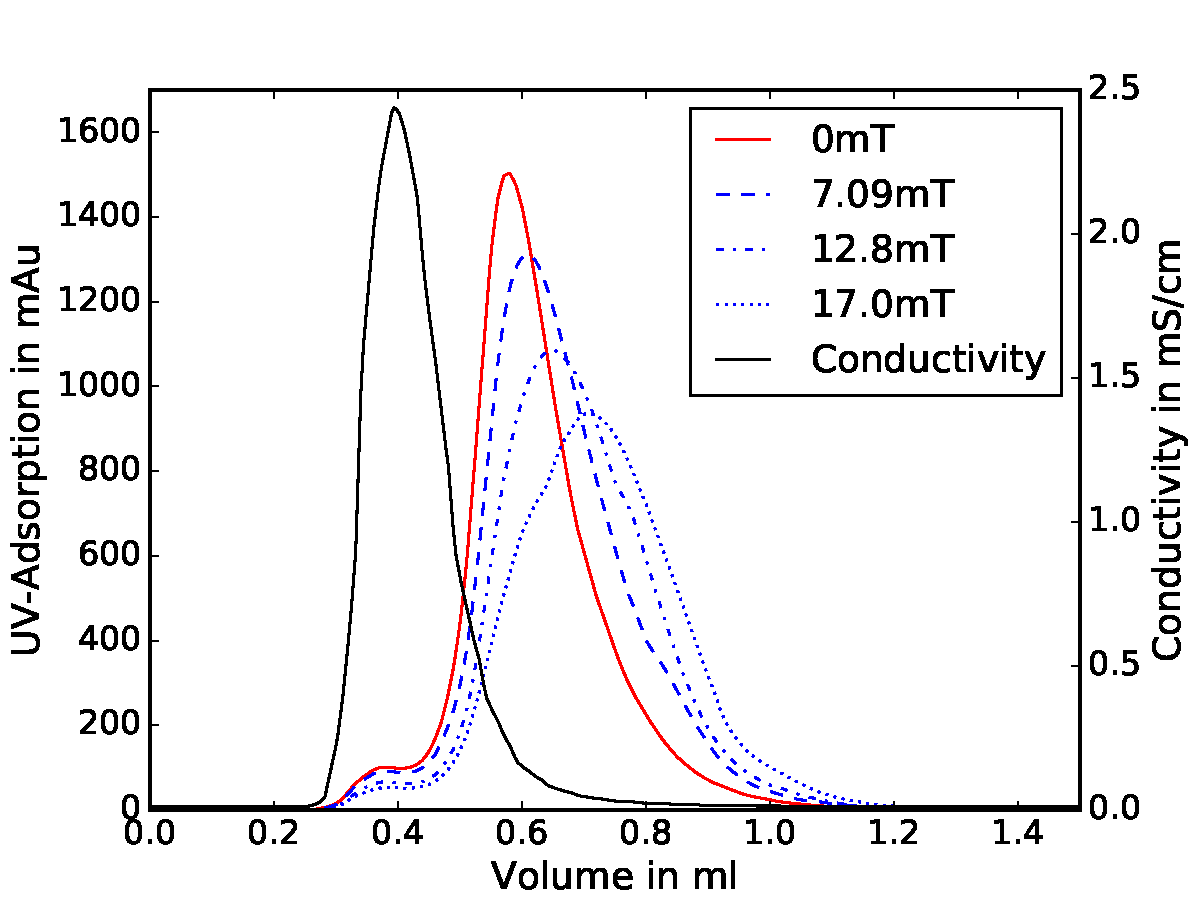
\includegraphics{figures/MF100_chemagen.pdf}}
                  \caption{}\label{subfig:sw_periodicBC_Rw_var}
          \end{subfigure}\hfill
          \\
            \begin{subfigure}{0.49\textwidth}
                  \flushleft
                  \scalebox{0.42}{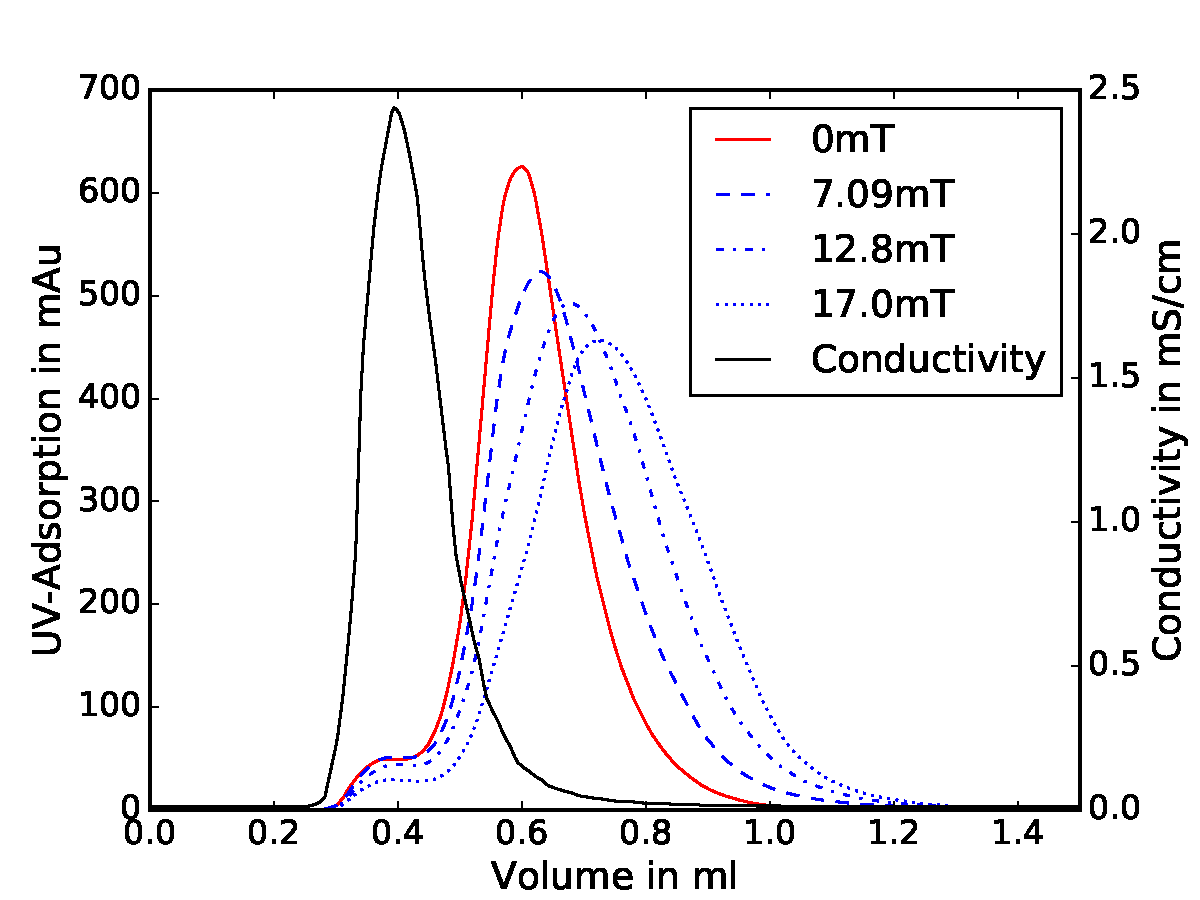
\includegraphics{figures/MF150_chemagen.pdf}}
                  \caption{}\label{subfig:sw_periodicBC_U0_var}
          \end{subfigure}\hfill
        \begin{subfigure}{0.49\textwidth}
                \flushright
                \scalebox{0.42}{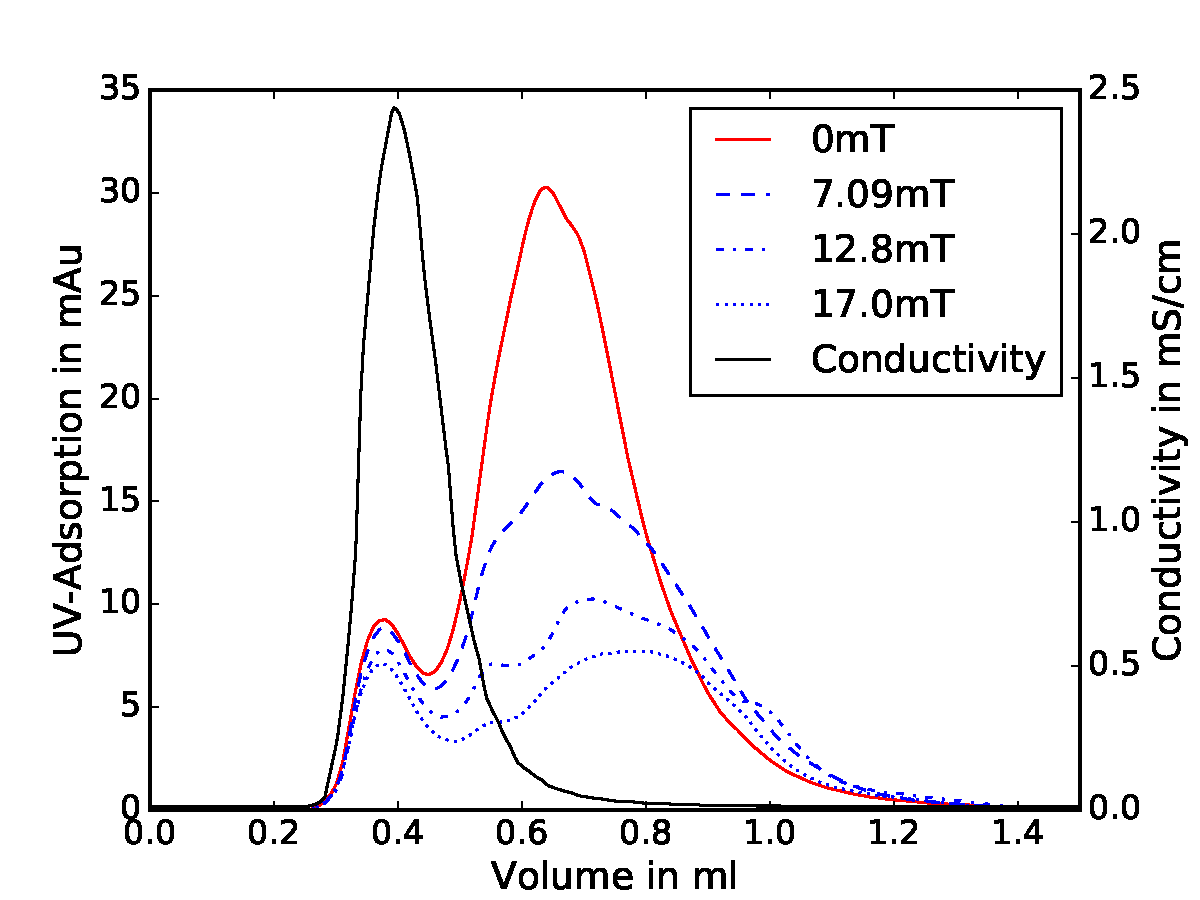
\includegraphics{figures/MF200_chemagen.pdf}}
                \caption{}\label{subfig:sw_periodicBC_Rp_var}
        \end{subfigure}
        \\
        
        \caption[]{}
        \label{fig:diff_conc_chemagen_peaks}
  \end{figure}        
		
\setcounter{figure}{0}
		
